\chapter{梯度感知的颜色分布映射方法}
本章内容概括。
\section{图像颜色编辑的梯度感知优化策略}
论文主体是毕业论文的主要部分,必须言之成理,论据可靠 \cite{tighe2013finding},严格遵循本学科国际通行的学术规范。在写作上要注意结构合理、层次分明、重点突出。

本章举例说明本模板中图片,表格及公式的插入及引用方法 \cite{liu2011sift}。

\subsection{图片格式举例}

图片的分辨率至少300个像素,建议格式为.png。图 \ref{fig1} 显示……,图 \ref{subfig1} 表明……。

\subsubsection{单张图片}
\begin{figure}[h]
	\centering
	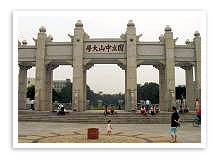
\includegraphics[width=0.8\textwidth]{figure/fig1.png}
	\caption{标题} 
	\label{fig1}
\end{figure}

\subsubsection{多张子图}
\begin{figure}[h!] % image examples & compare
	\begin{subfigure}{0.55\textwidth}
		\centering
		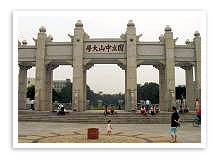
\includegraphics[width=0.5\textwidth]{figure/fig1.png}
		\caption{子图1}
		\label{subfig1}
	\end{subfigure}
	\begin{subfigure}{0.55\textwidth}
		\centering
		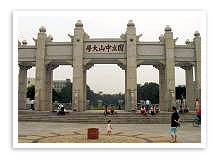
\includegraphics[width=0.5\textwidth]{figure/fig1.png} 
		\caption{子图2}
		\label{subfig2}
	\end{subfigure}
	\begin{subfigure}{0.55\textwidth}
		\centering
		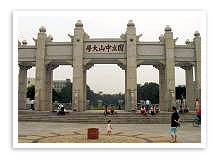
\includegraphics[width=0.5\textwidth]{figure/fig1.png}
		\caption{子图3}
		\label{subfig3}
	\end{subfigure}
	\begin{subfigure}{0.55\textwidth}
		\centering
		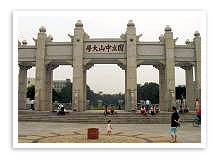
\includegraphics[width=0.5\textwidth]{figure/fig1.png} 
		\caption{子图4}
		\label{subfig4}
	\end{subfigure}
	\caption{多子图}
	\label{subfig}
\end{figure}




\subsection{表格举例}
表 \ref{tab1} 表示……。
\begin{table}[h]
	\centering
	\caption{国际单位制中具有专门名称的导出单位}		
	\label{tab1}
	\begin{tabular}{c|c|c|c}
		\toprule[2pt]
		量的名称 & 单位名称 & 单位符号 & 其他表示式例\\
		\midrule[2pt]
		频率	& 赫[兹]	& Hz	&$s^{-1}$ \\
		\hline                                        %细横线
		力;重力 	& 牛[顿]	& $N$	 & $kg·m/s^2$ \\
		\hline                                         %细横线
		压力,压强;应力	& 帕[斯卡]	&$Pa$	&$N/m^2$ \\
		\bottomrule[2pt]
	\end{tabular}
\end{table}

\subsection{公式举例}
\label{sec:formula}
没有编号的公式:
\begin{equation*}
\bm{z}^{(l)} = \bm{W}^{(l)}\bm{a}^{(l-1)} + \bm{b}^{(l)} 
\end{equation*}

公式中含有中文:
\begin{equation}
\mbox{像素准确率} = \sum_{i=1}^{n_{cl}}n_{ii} / \sum_{i=1}^{n_{cl}}t_i
\end{equation}

公式中含有矩阵:
\begin{equation}
\label{eq1}
\textbf{H} = \begin{bmatrix}
I*\bm{x}_i \\ \textbf{h}
\end{bmatrix}
\end{equation}

多行公式:
\begin{align} 
\hat{\bm{R}}_r 
& =   \frac{1}{N_s} \sum_{i=1}^{Ns} \bm{r}_i \bm{r}_i^T  \label{Eq-2-a} \\
& =   \frac{1}{N_s} \sum_{i=1}^{Ns} \bm{r}_i \bm{r}_i^T  \nonumber \\
& =   \frac{1}{N_s} \sum_{i=1}^{Ns} \bm{r}_i \bm{r}_i^T  \label{Eq-2-c},
\end{align}

引用:公式 \eqref{eq1} ……,\eqref{Eq-2-a}……。

更多的数学公式编辑方法,请参考根文件下“LaTex学习文档”中的文献1和文献3。

\subsection{算法举例}


\begin{algorithm}[h]
	\KwIn{$m$个训练样本}
	\lFor{$l=1$ \emph{\KwTo} $n_l$}{
		初始化:$\Delta \bm{W}^{(l)}=0$,$\Delta \bm{b}^{(l)}=0$}
	\ForEach{训练样本}{
		\lFor{$l=1$ \emph{\KwTo} $n_l-1$}{
			前向传播:$\bm{z}^{(l+1)}=\bm{W}^la^l+\bm{b}^l$,$\bm{a}^{(l+1)}=f(\bm{z}^{(l+1)})$}
		输出误差计算:$\delta^{(n_l)} = \frac{\partial}{\partial \bm{z}^{(n_l)}} J(\bm{W},\bm{b};\bm{x},y)$\;
		\lFor{$l=n_l-1$ \emph{\KwTo} $1$}{
			后向传播:$\delta^{(l)} = \bigl((\bm{W}^{(l)})^T \delta^{(l+1)}\bigr)f'(\bm{z}^{(l)})$}
		\ForAll{层l}{
			计算梯度:$\nabla_{\bm{W}^{(l)}}J(\bm{W},\bm{b};\bm{x},y)=\delta^{(l+1)}(\bm{a}^{(l)})^T$ \\
			\hspace{60pt}$\nabla_{\bm{b}^{(l)}}J(\bm{W},\bm{b};\bm{x},y)=\delta^{(l+1)}$\;
			累加梯度:$\Delta \bm{W}^{(l)} \leftarrow \Delta \bm{W}^{(l)} + \nabla_{\bm{W}^{(l)}}J(\bm{W},\bm{b};\bm{x},y)$; \\
			\hspace{60pt}$\Delta \bm{b}^{(l)} \leftarrow \Delta \bm{b}^{(l)} + \nabla_{\bm{b}^{(l)}}J(\bm{W},\bm{b};\bm{x},y)$\;
		}
	}
	\ForAll{层$l$}{
		更新权重:$\bm{W}^{(l)} \leftarrow \bm{W}^{(l)} - \alpha \biggl[\frac 1m \Delta \bm{W}^{(l)}]$ \\
		\hspace{60pt} $\bm{b}^{(l)} \leftarrow \bm{b}^{(l)} - \alpha \biggl[\frac 1m \Delta \bm{b}^{(l)}\biggr]$
	}
	\caption{梯度下降算法}
	\label{sgd}
\end{algorithm}

算法 \ref{sgd}……。

\subsection{例子}
\begin{eg}
	这是一个例子。
	\label{eg1}
\end{eg}
例 \ref{eg1} ……。

\subsection{证明}
\begin{proof}
证明过程
\end{proof}

\subsection{定理}
\begin{theorem}
	这是一个定理。
	\label{th1}
\end{theorem}
定理 \ref{th1} ……。

\subsection{命题}
\begin{proposition}
	这是一个命题。
	\label{pro1}
\end{proposition}
命题 \ref{pro1} ……。

\subsection{引理}
\begin{lemma}
	这是一个引理。
	\label{lem1}
\end{lemma}
引理 \ref{lem1} ……。

\subsection{推论}
\begin{corollary}
	这是一个推论。
	\label{cor1}
\end{corollary}
推论 \ref{cor1} ……。

\subsection{定义}
\begin{definition}
	这是一个定义。
	\label{def1}
\end{definition}
定义 \ref{def1} ……。

\subsection{标记}
\begin{remark}
	这是一个标记。
	\label{rem1}
\end{remark}
标记 \ref{rem1} ……。


\section{基于N维颜色直方图匹配的颜色映射方法}

\section{梯度感知的颜色分布映射方法}

\section{梯度感知的颜色分布映射方法实验结果分析}

\section{本章小结}